\chapter{Expansion Methods}
\label{sec:expansion_methods}

Expansion methods are series approximations of a probability density function. In general, these approximations are not true densities, as they can take negative values for certain parameter choices. However, for some parameter sets, they do define valid probability densities. In the following sections, we will explore the conditions under which expansion methods yield proper densities and how to transform a parameter set that does not correspond to a valid density into one that does.

\section{Gram-Charlier Expansion}
The Gram-Charlier expansion was introduced by Gram (\citeyear{gramUeberEntwickelungReeller1883}) and Charlier (\citeyear{charlierContributionsMathematicalTheory1914}). There are two types of expansions: Gram-Charlier A and Gram-Charlier B, which are defined as
\begin{align}
    f_{GC,A} &\approx f(x) + \sum_{k=3}^n a_k f^{(k)}(x) \notag \\
    f_{GC,B} &\approx \psi(x)\sum_{m=0}^n b_mg_m(x) \notag
\end{align}
Although these expansions can be applied to any density function $f$ and $\psi$, for Gram-Charlier Type A, the density $f$ is typically the standard normal distribution
\begin{align}
    f(x) = \frac{1}{\sqrt{2\pi}}\exp\left(-\frac{x^2}{2}\right) \notag
\end{align}
and for Gram-Charlier Type B, $\psi$ corresponds to the probability mass function of the Poisson distribution (\cite{mitropolskiiGramCharlierSeries2020}):
\begin{align}
    \psi(x) = \frac{\lambda^x}{x!}\exp(-\lambda) \notag
\end{align}
The term $f^{(k)}$ represents the $k$-th derivative of the density function $f$. There exist polynomials $H_k$ that satisfy
\begin{align}
    f^{(k)}(x) = (-1)^k f(x)H_k(x) \notag
\end{align}
These polynomials, known as Hermite polynomials, were studied by Laplace (\citeyear{laplaceMemoireIntegralesDefinies1811,laplaceTheorieAnalytiqueProbabilites1812}), Chebyshev (\citeyear{chebyshevDeveloppementFonctionsSeule1860}), and Hermite (\citeyear{hermiteNouveauDeveloppementSerie1864}). They have the following properties (\cite{abramowitzHandbookMathematicalFunctions1968}, p. 771ff):
\begin{align}
    H_{n+1} &= x\cdot H_n(x) - H'_n(x) \notag \\
    H'_n(x) &= n\cdot H_{n-1}(x) \notag \\
\end{align}
Using these recurrence relations, the first few Hermite polynomials can be computed as
\begin{align}
    H_{n+1}(x) &= x\cdot H_n(x) - nH_{n-1}(x) \notag \\
    H_0(x) &= 1 \notag \\
    H_1(x) &= x \notag \\
    H_2(x) &= x^2 - 1 \notag \\
    H_3(x) &= x^3-3x \notag \\
    H_4(x) &= x^4-6x^2+3 \notag \\
    H_5(x) &= x^5-10x^3+15x \notag \\
    H_6(x) &= x^6-15x^4+45x^2-15 \notag
\end{align}
The coefficients $a_k$ in the expansion can be expressed in terms of the moments $r_k$ of the density $f$. This leads to the first terms of the Gram-Charlier A expansion:
\begin{align}
    \label{eq:gc_a_expansion_kappa}
    f(x)_{GC,A} \approx &\, \frac{1}{\sqrt{2\pi}\sigma}\exp\left(-\frac{(x-\mu)^2}{2\sigma^2}\right) \notag\\[1ex]
    &\, \times \left[1 + \frac{\kappa_3}{6\sigma^3}H_3\left(\frac{x-\mu}{\sigma}\right)
    + \frac{\kappa_4}{24\sigma^4}H_4\left(\frac{x-\mu}{\sigma}\right)\right]
\end{align}
where $\mu$, $\sigma^2$, $\kappa_3$, and $\kappa_4$ represent the first four cumulants of the target distribution. Based on Equations \eqref{eq:cumulants_1} and \eqref{eq:cumulants_2}, $\mu$ and $\sigma^2$ correspond to the first two cumulants $\kappa_1$ and $\kappa_2$.

The first terms of the Gram-Charlier B expansion are given by
\begin{align}
    f(x)_{GC,B} \approx &\; \frac{\lambda^x}{x!}\exp(-\lambda) \notag\\[1ex]
    &\; \times \Biggl( 1 
       + \frac{\mu_2 - \lambda}{\lambda^2}\Bigl[\frac{x^{[2]}}{2} - \lambda x^{[1]} + \frac{\lambda^2}{2}\Bigr] \notag\\[1ex]
    &\quad + \frac{\mu_3 - 3\mu_2 + 2\lambda}{\lambda^3}\Bigl[\frac{x^{[3]}}{6} - \frac{\lambda}{2}x^{[2]} + \frac{\lambda^2}{2}x^{[1]} - \frac{\lambda^3}{6}\Bigr] \Biggr) \notag
\end{align}    
where $\mu_i$ are the central moments of the target distribution, and $x^{[i]} = x(x-1)\dots (x-i+1)$ (\cite{mitropolskiiGramCharlierSeries2020}). However, since Gram-Charlier Type B only allows discrete values for $x$, it cannot be applied to continuous distributions. Therefore, we focus exclusively on Gram-Charlier Type A in this work.

The Gram-Charlier expansion is not an asymptotic expansion, as it does not allow for a well-defined approximation error. The Edgeworth expansion, however, is an asymptotic expansion (\cite{cramerMathematicalMethodsStatistics1999}, Section 17.6) and is therefore preferred. An asymptotic expansion consists of a series of functions $f_n$ that, after a finite number of terms, approximate a function at a specific point $\xi$ (often infinite) as $x$ approaches $\xi$:
\begin{align}
    f_{n+1}(x) = \mathcal{o}(f_n(x)) \quad x\to\xi \notag
\end{align}
Furthermore, the Gram-Charlier expansion can take negative values, which is not permissible for a probability density function. Jondeau \& Rockinger (\citeyear{jondeauGramCharlierDensities2001}) analyzed the conditions under which the expansion remains a valid density. By using Equations \eqref{eq:cumulants_3} and \eqref{eq:cumulants_4}, Equation \eqref{eq:gc_a_expansion_kappa} can be rewritten in terms of the skewness $\gamma_1$ and excess kurtosis $\gamma_2^*$, defining $z = \frac{x-\mu}{\sigma}$:
\begin{align}
    \label{eq:gc_a_expansion_s_ek}
    f(x)_{GC,A} \approx \frac{1}{\sqrt{2\pi}}\exp\left(-\frac{z^2}{2}\right) \left[1 + \frac{\gamma_1}{6}H_3(z) + \frac{\gamma_2^*}{24}H_4(z)\right]
\end{align}
To determine when the Gram-Charlier expansion remains a valid density, the following condition must hold:
\begin{align}
    1 + \frac{\gamma_1}{6}He_3(z) + \frac{\gamma_2^*}{24}He_4(z) &= 0 \notag \\
    \frac{\gamma_1}{6}He_3(z) &= -1 - \frac{\gamma_2^*}{24}He_4(z) \notag \\
    \gamma_1\cdot He_3(z) &= -6 - \frac{\gamma_2^*}{4}He_4(z) \notag \\
    \gamma_1 &= -\frac{6}{He_3(z)} - \frac{He_4(z)}{4\cdot He_3(z)}\gamma_2^* \notag \\
    \gamma_1 &= \frac{z^4-6z^2+3}{12z-4z^3}\cdot \gamma_2^* + \frac{24}{12z-4z^3} \notag
\end{align}
This leads to a boundary condition for the skewness and excess kurtosis, illustrated in Figures \ref{fig:gram_charlier_boundary_lines_20_vs_1000} and \ref{fig:gram_charlier_boundary}.

Using a bisection algorithm and a logistic mapping, Jondeau \& Rockinger (\citeyear{jondeauGramCharlierDensities2001}) construct a piecewise linear boundary, ensuring that any unconstrained pair $(\tilde{\gamma_1}, \tilde{\gamma_2^*}) \in \mathbb{R}^2$ is mapped to a constrained pair within the positivity region $\mathcal{D}$. Finding a closed-form expression for the boundary is computationally difficult; even with 24 hours on a high-performance computer using Python's SymPy library, no explicit solution was found.

A comparison between constrained and unconstrained parameters for four distributions—standard normal, lognormal, $t$-distribution, and non-central $t$-distribution—is presented in Table \ref{table:distributions_theoretical_moments} and Figures \ref{fig:gc_expansion} and \ref{fig:gc_positivity_expansion}. The results highlight the necessity of positivity constraints, which, however, distort the expansion, particularly for cases where no constraints were originally required (e.g., the standard normal distribution). The logistic mapping shifts the excess kurtosis from 0 to 2, mapping the unconstrained pair $(\tilde{\gamma_1}, \tilde{\gamma_2^*}) = (0,0)$ to the constrained pair $(\gamma_1, \gamma_2^*) = (0,2)$.

\begin{figure}[h]
    \centering
    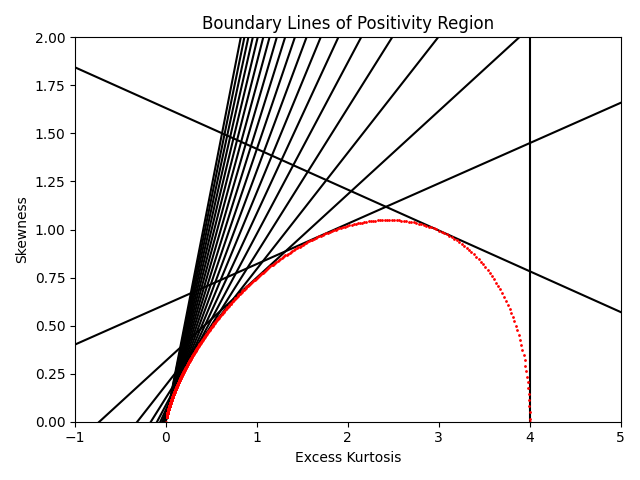
\includegraphics[width=0.4\textwidth]{img/gc_positivity_boundary_lines_20.png}
    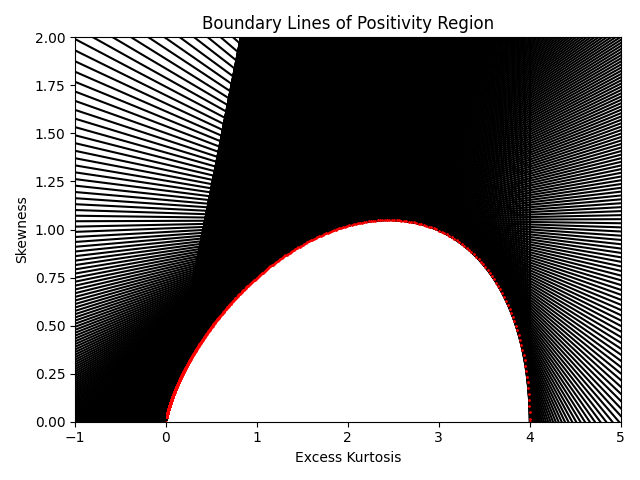
\includegraphics[width=0.4\textwidth]{img/gc_positivity_boundary_lines_1000.png}
    \caption{Boundary lines of the positivity region of the Gram-Charlier Expansion. The left image shows 20 lines, the right image shows 1000 lines. The red dots are the boundary points. The boundary is symmetric to the x-axis.}
    \label{fig:gram_charlier_boundary_lines_20_vs_1000}
\end{figure}

\begin{figure}[h]
    \centering
    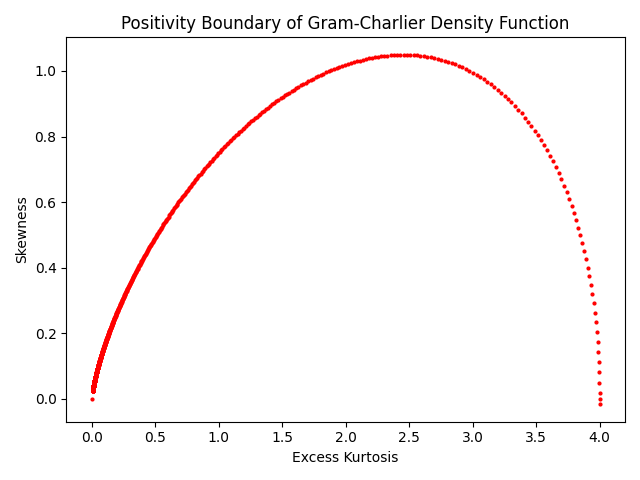
\includegraphics[width=0.8\textwidth]{img/gc_positivity_boundary.png}
    \caption{Approximation (1000 steps) of the positivity boundary of the Gram-Charlier Expansion. For simplicity, only the part above the x-axis is shown. The boundary is symmetric to the x-axis.}
    \label{fig:gram_charlier_boundary}
\end{figure}

\begin{table}[h]
    \centering
    \begin{tabular}{l|l|l|l|l|l|l|l}
        Distribution & $\mu$ & $\sigma^2$ & $\kappa_3$ & $\gamma_1$ & $\kappa_4$ & $\gamma_2^*$ \\
        \hline
        $\mathcal{N}(\mu=0,\sigma1)$ & 0 & 1 & 0 & 0 & 0 & 0 \\
        $\mathcal{L}(\mu=0, \sigma=0.5)$ & 1.1331 & 0.3647 & 0.3855 & 1.7502 & 0.7845 & 5.8984 \\
        $\mathcal{T}(\nu=5)$ & 0 & 1.6667 & 0 & 0 & 16.6667 & 6 \\
        $\mathcal{NCT}(\nu=5, \mu=0.5)$ & 0.5947 & 1.7297 & 1.5357 & 0.6751 & 21.5969 & 7.2189
    \end{tabular}
    \caption{Distribution parameters and theoretical moments and cumulants. $\mathcal{N}$ stands for the Normal distribution, $\mathcal{L}$ for the Lognormal distribution, $\mathcal{T}$ for the Student's $t$-distribution, and $\mathcal{NCT}$ for the Non-Central $t$-distribution.}
    \label{table:distributions_theoretical_moments}
\end{table}

\begin{figure}[h]
    \centering
    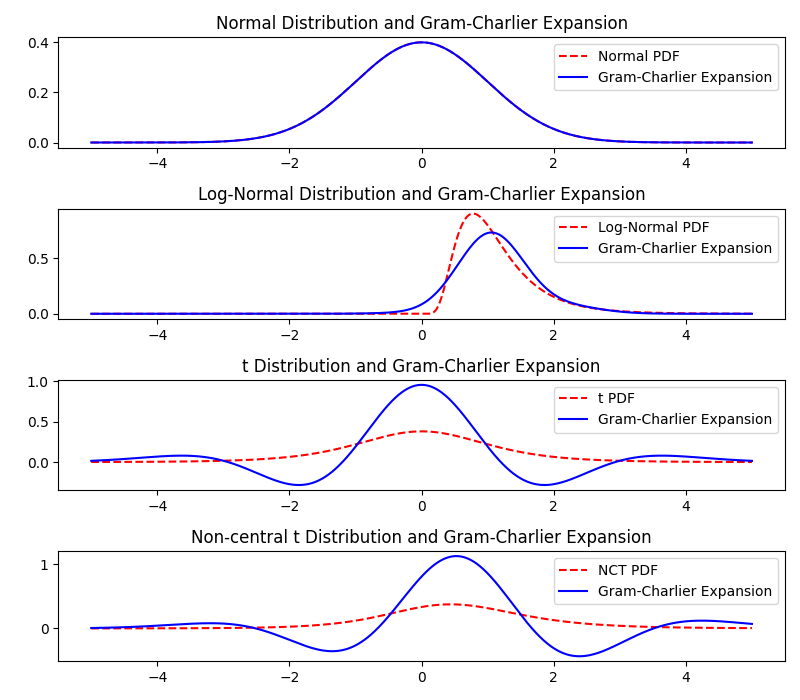
\includegraphics[width=0.8\textwidth]{img/gc_expansion.png}
    \caption{Gram-Charlier Expansion of different distributions}
    \label{fig:gc_expansion}
\end{figure}

\begin{figure}[h]
    \centering
    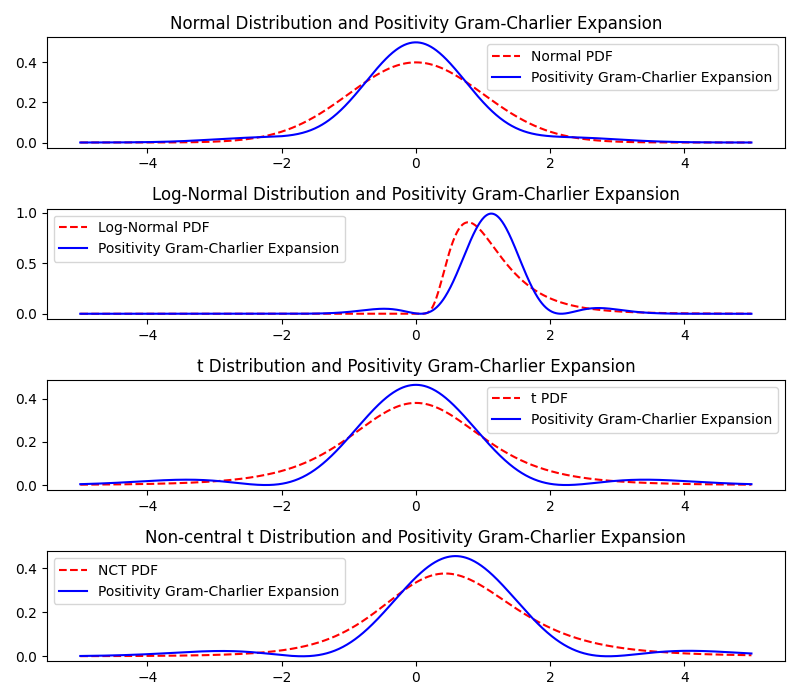
\includegraphics[width=0.8\textwidth]{img/gc_positivity_expansion.png}
    \caption{Gram-Charlier Expansion with positivity constraints of different distributions}
    \label{fig:gc_positivity_expansion}
\end{figure}

\section{Edgeworth Expansion}
Originally introduced by Edgeworth \citeyear{edgeworthRepresentationStatisticalFrequency1907}, who suggested computing the approximation up to the sixth term to mitigate the issues associated with asymptotic expansions. A formal representation of the first terms can be found in Brenn \& Anfinsen (\citeyear{brennRevisitGramCharlierEdgeworth2017}).
\begin{align}
    f(x)_{EW} \approx &\; \frac{1}{\sqrt{2\pi}\sigma}\exp\left(-\frac{(x-\mu)^2}{2\sigma^2}\right) \notag\\[1ex]
    &\; \times \Biggl[ 1 
        + \frac{\kappa_3}{6\sigma^3}H_3\left(\frac{x-\mu}{\sigma}\right) + \frac{\kappa_4}{24\sigma^4}H_4\left(\frac{x-\mu}{\sigma}\right) \notag\\[1ex]
    &\quad + \frac{\kappa_5}{120\sigma^5}H_5\left(\frac{x-\mu}{\sigma}\right) + \frac{\kappa_6 + 10\kappa_3^2}{720\sigma^6}H_6\left(\frac{x-\mu}{\sigma}\right)
    \Biggr] \notag
\end{align}
    
Since this work only considers the first four cumulants, the expression simplifies to:
\begin{align}
    f(x)_{EW} \approx {} & \frac{1}{\sqrt{2\pi}\sigma}\exp\left(-\frac{(x-\mu)^2}{2\sigma^2}\right)\notag\\[1ex]
    & \quad \times \Biggl[ 1 
       + \frac{\kappa_3}{6\sigma^3}H_3\left(\frac{x-\mu}{\sigma}\right) + \frac{\kappa_4}{24\sigma^4}H_4\left(\frac{x-\mu}{\sigma}\right) \notag\\[1ex]
    \label{eq:ew_expansion_short}
    & \quad \quad + \frac{\kappa_3^2}{72\sigma^6}H_6\left(\frac{x-\mu}{\sigma}\right)
    \Biggr]
\end{align}    

Following the approach of Jondeau \& Rockinger (\citeyear{jondeauGramCharlierDensities2001}) for the Gram-Charlier expansion, we determine the positivity boundary for the Edgeworth expansion by rewriting Equation \eqref{eq:ew_expansion_short} using $z = \frac{x-\mu}{\sigma}$:
\begin{align}
    \label{eq:ew_expansion_s_ek}
    f(x)_{EW} \approx \frac{1}{\sqrt{2\pi}}\exp\left(-\frac{z^2}{2}\right) \left[1 + \frac{\gamma_1}{6}H_3(z) + \frac{\gamma_2^*}{24}H_4(z) + \frac{\gamma_1^2}{72}He_6(z)\right]
\end{align}
To ensure the expansion remains a valid density, we solve for skewness $\gamma_1$ in the equation:
\begin{align}
    0 &= 1+\frac{\gamma_1}{6}He_3(z) + \frac{\gamma_2^*}{24}He_4(z) + \frac{\gamma_1^2}{72}He_6(z) \\
    \gamma_1 &= \pm\sqrt{-\frac{72}{He_6(z)} - 3\gamma_2^*\frac{He_4(z)}{He_6(z)} + 36\frac{He_3(z)^2}{He_6(z)^2}} - 6\frac{He_3(z)}{He_6(z)} \notag
\end{align}
This equation is valid as long as $H_6(z) \neq 0$, which occurs at six points:
\begin{align}
    z_{1/2} &= \pm \sqrt{5-\frac{5^{2/3}\left(1+i\sqrt{3}\right)}{\sqrt[3]{2\left(2+i\sqrt{6}\right)}} - \frac{\left(1-i\sqrt{3}\right)\sqrt[3]{5\left(2+i\sqrt{6}\right)}}{2^{2/3}}} = \pm 0.6167 \notag\\
    z_{3/4} &= \pm \sqrt{5-\frac{5^{2/3}\left(1-i\sqrt{3}\right)}{\sqrt[3]{2\left(2+i\sqrt{6}\right)}} - \frac{\left(1+i\sqrt{3}\right)\sqrt[3]{5\left(2+i\sqrt{6}\right)}}{2^{2/3}}} = \pm 1.8892 \notag \\
    z_{5/6} &= \pm \sqrt{5+\frac{10^{2/3}}{\sqrt[3]{2+i\sqrt{6}}} + \sqrt[3]{10\left(2+i\sqrt{6}\right)}} = \pm 3.3243 \notag
\end{align}

\begin{figure}[h]
    \centering
    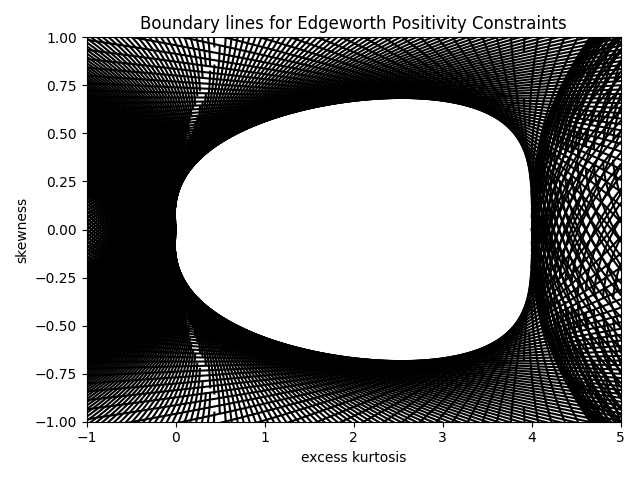
\includegraphics[width=0.8\textwidth]{img/edgeworth_positivity_boundary_lines.png}
    \caption{Boundary Lines for Edgeworth Expansion}
    \label{fig:ew_boundary_lines}
\end{figure}
\begin{figure}[h]
    \centering
    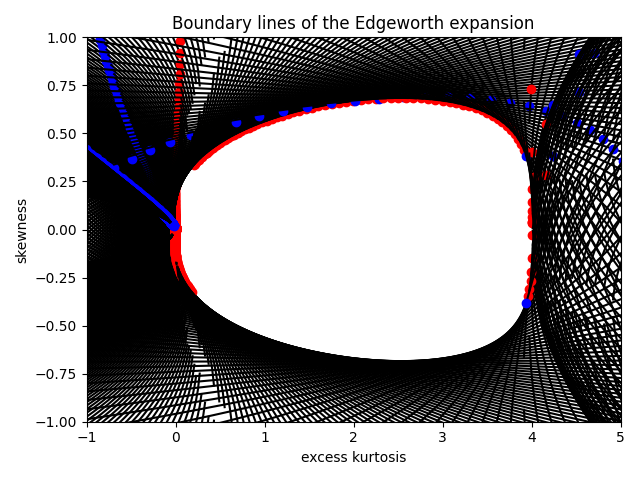
\includegraphics[width=0.8\textwidth]{img/edgeworth_positivity_boundary_intersections_1.png}
    \caption{Intersections of Boundary Lines for Edgeworth Expansion, red is first intersection, blue is second intersection}
    \label{fig:ew_boundary_intersections_1}
\end{figure}
\begin{figure}[h]
    \centering
    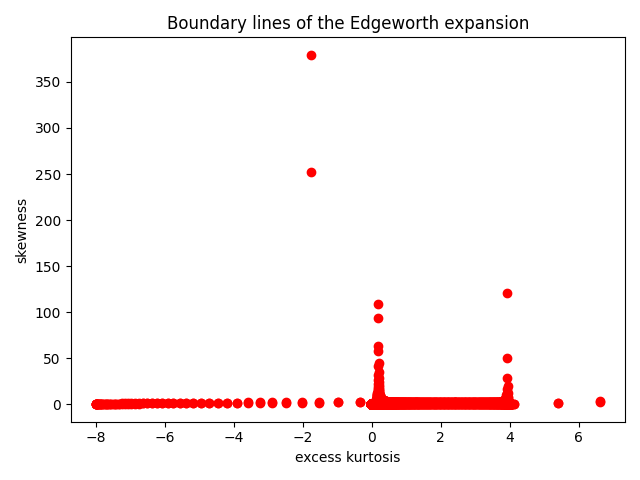
\includegraphics[width=0.8\textwidth]{img/edgeworth_positivity_boundary_intersections_3.png}
    \caption{Intersections of Boundary Lines for Edgeworth Expansion (zoomed out), upper half}
    \label{fig:ew_boundary_intersections_3}
\end{figure}
\begin{figure}[h]
    \centering
    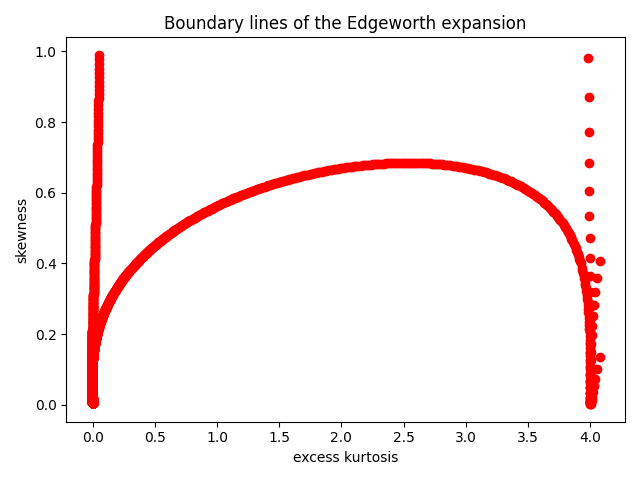
\includegraphics[width=0.8\textwidth]{img/edgeworth_positivity_boundary_intersections_4.png}
    \caption{Intersections of Boundary Lines for Edgeworth Expansion (zoomed in), upper half}
    \label{fig:ew_boundary_intersections_4}
\end{figure}
\begin{figure}[h]
    \centering
    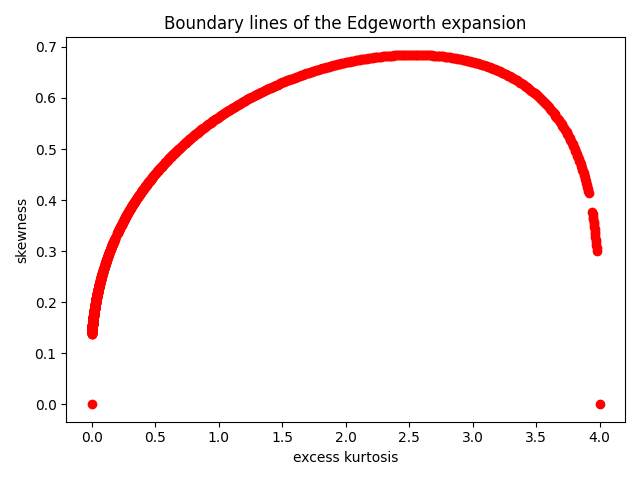
\includegraphics[width=0.8\textwidth]{img/edgeworth_positivity_boundary_intersections_7.png}
    \caption{Final Boundary Points for Edgeworth Expansion, upper half}
    \label{fig:ew_boundary_intersections_7}
\end{figure}

The positivity boundary for the Edgeworth expansion is determined by plotting the lines $\gamma_1(\gamma_2^*, z)$ for many values of $z$, skipping over the six singularities. Figure \ref{fig:ew_boundary_lines} shows that the positivity region for the Edgeworth expansion is smaller than for the Gram-Charlier expansion. For $\gamma_1 = 0$, the excess kurtosis is constrained between 0 and 4, which matches the boundary of the Gram-Charlier expansion since both expansions are identical when skewness is zero.

As with the Gram-Charlier expansion, the positivity boundary is given by the envelope of the lines $\gamma_1(\gamma_2^*, z)$. We obtain this by computing the intersections of pairs of parabolic equations. The equations are to long to be displayed here, you can find them in the corresponding GitHub repository\footnote{\url{https://github.com/henrydatei/heston-moments-pdf}}. These intersections are shown in Figures \ref{fig:ew_boundary_intersections_1} to \ref{fig:ew_boundary_intersections_7}.

Since each $\gamma_1(\gamma_2^*, z)$ equation is a parabola, the positivity region can be computed by:
\begin{enumerate}
    \item Ignoring the second intersection for each $z$-value (since the first intersection defines the boundary). The boundary is symmetric around the $x$-axis, so we only compute the upper half and mirror it afterward.
    \item Filtering out non-relevant points: Figure \ref{fig:ew_boundary_intersections_3} shows many extraneous intersection points. Based on previous results, we restrict the solutions to $\gamma_2^* \in (-0.1,4.1)$ and $\vert \gamma_1\vert \in [0,1)$. (see Figure \ref{fig:ew_boundary_intersections_4})
    \item Removing points from non-relevant boundary lines: The lower-boundary artifacts arise from $z$-values smaller than the third singularity; these are removed. The upper-boundary artifacts come from $\vert z \vert$ around 1.8 and 1.67, and are filtered out by removing all $z$ in the ranges $(1.8-0.035, 1.8+0.035)$ and $(1.67-0.015,1.67+0.015)$.
    \item Computational accuracy is a concern since some points lie slightly outside the expected range (e.g., one point is at $(\gamma_2^*, \gamma_1) = (4.01, 0.222)$). Testing this point in the Edgeworth expansion shows that it does not satisfy the positivity condition:
    \begin{align}
        1 + \frac{0.222}{6}He_3(z) + \frac{4.01}{24}He_4(z) + \frac{0.222^2}{72}He_6(z)<0 \notag
    \end{align}
    gives a solution: $-1.84611<z<-1.75826$. This might be due to Python's float datatype which maps to IEEE-754 double precision with 64 bits where 52 bits are used for the fraction which equals about 16 decimal digits (\cite{pythonfoundation15FloatingPointArithmetic,leonardo.zAnswerHowCan2013}) To be conservative, we remove any intersection with $\gamma_2^* \notin [0,4]$.
    \item Adding the points $(0,0)$ and $(4,0)$ completes the positivity region. A linear interpolation between the closest computed boundary points results in the final positivity boundary (see Figure \ref{fig:ew_boundary_intersections_7}).
\end{enumerate}

\begin{figure}[h]
    \centering
    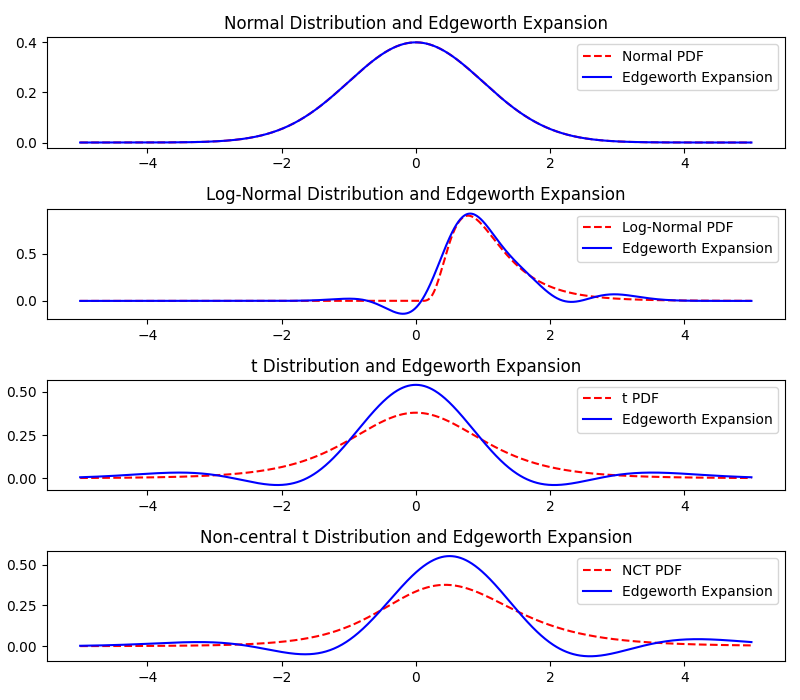
\includegraphics[width=0.8\textwidth]{img/ew_expansion.png}
    \caption{Edgeworth Expansion of different distributions}
    \label{fig:ew_expansion}
\end{figure}

\begin{figure}[h]
    \centering
    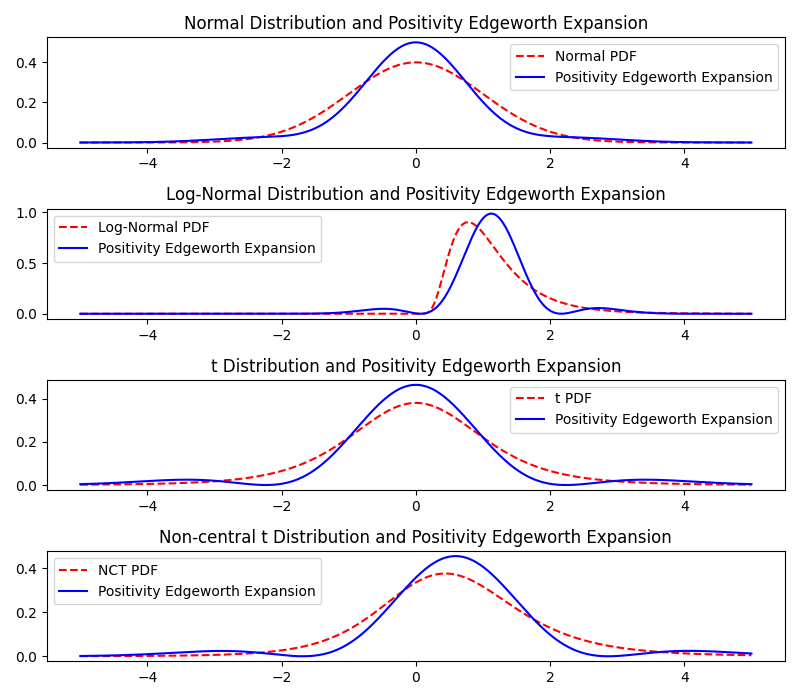
\includegraphics[width=0.8\textwidth]{img/ew_positivity_expansion.png}
    \caption{Edgeworth Expansion with positivity constraints of different distributions}
    \label{fig:ew_positivity_expansion}
\end{figure}

As with the Gram-Charlier expansion, we compare the constrained and unconstrained parameters for four distributions: standard normal, lognormal, $t$-distribution, and non-central $t$-distribution (see Table \ref{table:distributions_theoretical_moments}). The results, shown in Figures \ref{fig:ew_expansion} and \ref{fig:ew_positivity_expansion}, lead to the same conclusion as in the Gram-Charlier case: Positivity constraints are necessary, but they also distort the expansion and even when constraints are not needed (e.g., for the standard normal distribution), applying the positivity constraints artificially increases excess kurtosis from 0 to 2.

\section{Cornish-Fisher Expansion}

The Cornish-Fisher expansion, introduced by Cornish and Fisher (\citeyear{cornishMomentsCumulantsSpecification1938}), is an asymptotic expansion that approximates the quantiles of a probability distribution based on its cumulants.

Given that $z_p$ is the $p$-quantile of a normal distribution with mean $\mu$ and variance $\sigma^2$, the $p$-quantile of a random variable $X$, denoted as $x_p$, can be approximated as follows (only the first terms shown, as it is common practice) (\cite{abramowitzHandbookMathematicalFunctions1968}, p. 935):
\begin{align}
    x_p \approx z_p + \frac{\gamma_1}{6}He_2(z_p) + \frac{\gamma_2^*}{24}He_3(z_p) - \frac{\gamma_1^2}{36}(2\cdot He_3(z_p) + He_1(z_p)) \notag
\end{align}
To obtain the probability density function (PDF), the quantiles $x_p$ can be numerically computed and differentiated.

Aboura \& Maillard (\citeyear{abouraOptionPricingSkewness2016}) point out that the parameters $\gamma_1$ and $\gamma_2^*$ do not correspond to the skewness and excess kurtosis of the approximated distribution. Instead, they denote these parameters as $s = \gamma_1$ and $k = \gamma_2^*$ and provide equations to compute the actual skewness $s^*$ and excess kurtosis $k^*$ of the approximated distribution:
\begin{align}
    s^* &= \frac{M_3}{M_{2}^{3/2}} \notag \\
    k^* &= \frac{M_4}{M_{2}^2} - 3 \notag \\
    M_1 &= 0 \\
    M_2 &= 1 + \frac{1}{96}k^2 + \frac{25}{1296}s^4 - \frac{1}{36}ks^2 \\
    M_3 &= s - \frac{76}{216}s^3 + \frac{85}{1296}s^5 + \frac{1}{4}ks - \frac{13}{144}ks^3 + \frac{1}{32}k^2s \\
    M_4 &= 3 + k + \frac{7}{16}k^2 + \frac{3}{32}k^3 + \frac{31}{3072}k^4 - \frac{7}{216}s^4 - \frac{25}{486}s^6 + \frac{21665}{559872}s^8 \notag
\end{align}
Later, Maillard (\citeyear{maillardUserGuideCornish2018}) published the inverse transformation, allowing one to compute the parameters $s$ and $k$ given the actual skewness and excess kurtosis. A corresponding table can be found in the appendix of his paper.

Aboura \& Maillard (\citeyear{abouraOptionPricingSkewness2016}) also investigate the domain of validity for the Cornish-Fisher expansion. Their findings suggest that the expansion is valid for a wide range of parameters—even an excess kurtosis above 40 and skewness exceeding $\pm3$ are possible. However, when operating outside the validity domain, the issue is not immediately apparent in the probability density function itself. Instead, it becomes visible in the quantiles, which can turn negative (see Figures \ref{fig:cf_expansion} and \ref{fig:cf_expansion_cdf}).

\begin{figure}[h]
    \centering
    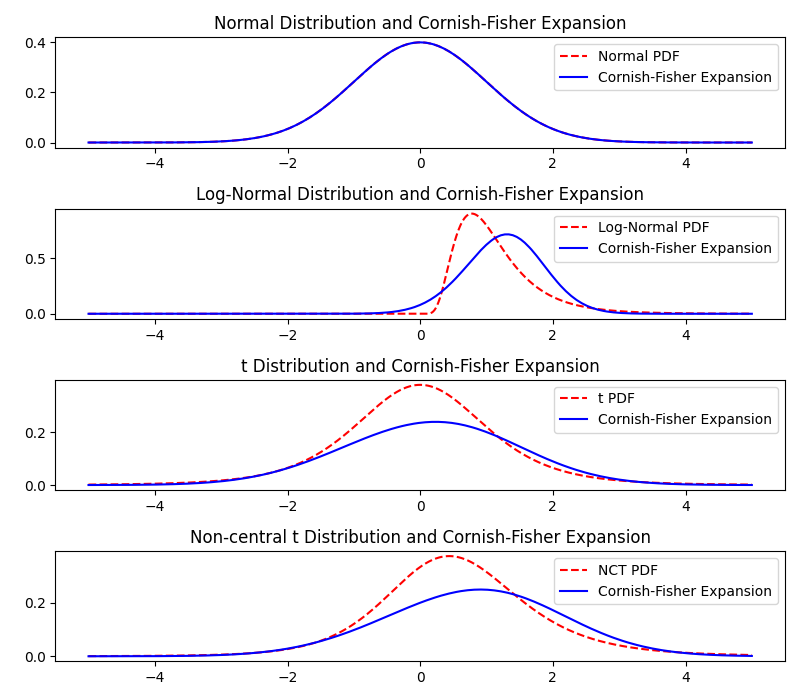
\includegraphics[width=0.8\textwidth]{img/cf_expansion.png}
    \caption{Cornish-Fisher Expansion of different distributions}
    \label{fig:cf_expansion}
\end{figure}

\begin{figure}[h]
    \centering
    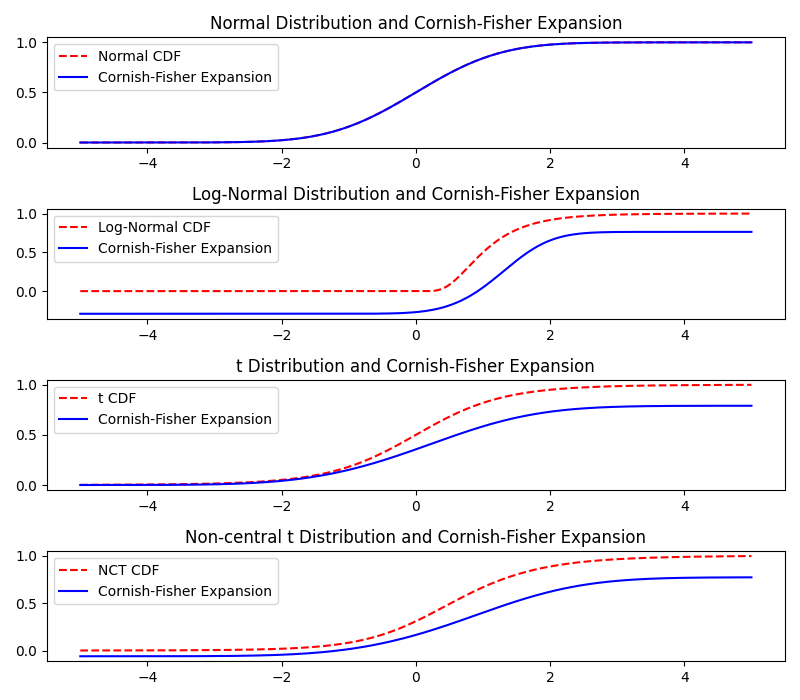
\includegraphics[width=0.8\textwidth]{img/cf_expansion_cdf.png}
    \caption{CDF of Cornish-Fisher Expansion of different distributions}
    \label{fig:cf_expansion_cdf}
\end{figure}

\section{Saddlepoint Approximation}

The Saddlepoint Approximation, introduced by Daniels (\citeyear{danielsSaddlepointApproximationsStatistics1954}), provides an accurate method for approximating probability densities. While Daniels initially derived the density function, the cumulative distribution function (CDF) was later introduced by Lugannani \& Rice (\citeyear{lugannaniSaddlePointApproximation1980}). This method is based on the moment generating function (MGF) and offers a highly precise approximation formula. Given that $M(t)$ is the moment generating function and $K(t) = \log(M(t))$ is the cumulant generating function, the approximation of the density function $f(x)$ is given by:
\begin{align}
    \label{eq:sp_approximation}
    f(x)_{SP} \approx \frac{1}{\sqrt{2\pi\cdot K''(s)}}\exp(K(s) - s\cdot x)
\end{align}
where $s$ is the solution of the equation $K'(s) = x$.

By definition, the cumulant generating function $K(s)$ can be approximated as:
\begin{align}
    K(s) \approx \kappa_1 s + \frac{\kappa_2 s^2}{2} + \frac{\kappa_3 s^3}{6} + \frac{\kappa_4 s^4}{24}
\end{align}
with its first and second derivatives:
\begin{align}
    K'(s) &= \kappa_1 + \kappa_2 s + \frac{\kappa_3 s^2}{2} + \frac{\kappa_4 s^3}{6} \notag \\
    K''(s) &= \kappa_2 + \kappa_3 s + \frac{\kappa_4 s^2}{2} \notag
\end{align}
To find $s$, we solve the equation $K'(s) = x$ under different conditions:
\begin{enumerate}
    \item If $\kappa_4 = 0$, $\kappa_3 = 0$, $\kappa_2 = 0$, and $\kappa_1 \neq 0$: No real solution exists.
    \item If $\kappa_4 = 0$, $\kappa_3 = 0$, and $\kappa_2 \neq 0$: A direct solution is given by:
    \begin{align}
        s = \frac{z-\kappa_1}{\kappa_2} \notag
    \end{align}
    \item If $\kappa_4 = 0$ and $\kappa_3 \neq 0$: The equation becomes quadratic, yielding two solutions:
    \begin{align}
        s = \frac{\pm\sqrt{-2\kappa_1\kappa_3 + 2\kappa_3 z + \kappa_2^2} - \kappa_2}{\kappa_3} \notag
    \end{align}
    \item If $\kappa_4 \neq 0$, then three solutions exist, two of which are complex, and one is real which is given by
    \begin{align}
        s &= \frac{1}{3\sqrt[3]{2}\kappa_4}\,\sqrt[3]{\Delta} - \frac{\sqrt[3]{2}\,(18\kappa_4\kappa_2-9\kappa_3^2)}{3\kappa_4\,\sqrt[3]{\Delta}} - \frac{\kappa_3}{\kappa_4} \notag \\
        \Delta &:= \sqrt{(-162\kappa_4^2\kappa_1 + 162\kappa_4^2x + 162\kappa_4\kappa_3\kappa_2 - 54\kappa_3^3)^2 + 4(18\kappa_4\kappa_2 - 9\kappa_3^2)^3} \notag\\[1ex]
        &\quad - 162\kappa_4^2\kappa_1 + 162\kappa_4^2x + 162\kappa_4\kappa_3\kappa_2 - 54\kappa_3^3 \notag
    \end{align}        
\end{enumerate}

\begin{figure}[h]
    \centering
    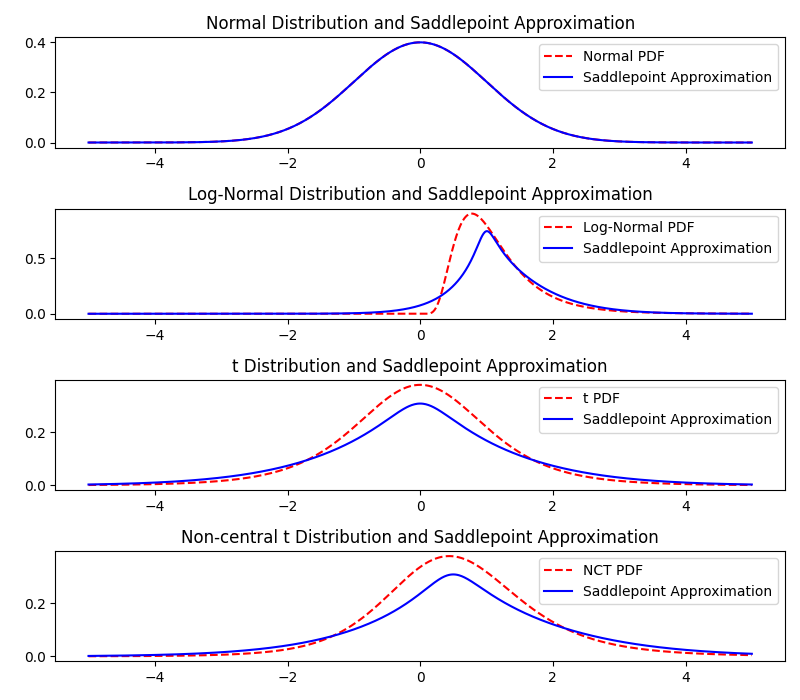
\includegraphics[width=0.8\textwidth]{img/saddle_approximation.png}
    \caption{Saddlepoint Approximation of different distributions}
    \label{fig:sp_approximation}
\end{figure}

The Saddlepoint Approximation successfully approximates the chosen distributions (see Table \ref{table:distributions_theoretical_moments}), as shown in Figure \ref{fig:sp_approximation}. The key advantages of this method are the high accuracy: The Saddlepoint method provides excellent approximations, even in cases where other expansions (such as Gram-Charlier or Edgeworth) fail. Furthermore there are no issues with negativity: The Saddlepoint Approximation does not produce negative densities. This is because the $\exp(\cdot)$ term in Equation \eqref{eq:sp_approximation} is always positive, and the denominator involves a square root, which is either positive or complex. If complex, the approximation does not exist, rather than producing invalid results.
